\documentclass{article}
\usepackage{amsmath}
\usepackage{amssymb}
\usepackage{graphicx}
\usepackage{hyperref}
\usepackage[version=4]{mhchem}


\begin{document}
(AMC) Medians \(B D\) and \(C E\) of a triangle \(A B C\) are perpendicular, \(B D\) \(=8\), and \(C E=12\). Find the area of triangle \(A B C\).

Solution: 64.
We draw the third median \(A F\).\\
\centering
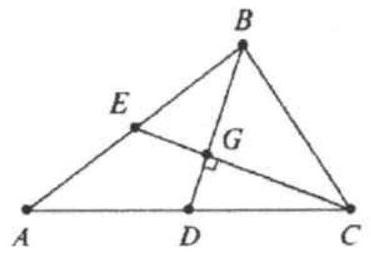
\includegraphics[width=\textwidth]{images/010(3).jpg}


\(C D=C D=\frac{1}{2} C M=\frac{4}{2}=2\).


\end{document}
